% !TeX spellcheck = en_US
\documentclass[aspectratio=1610]{beamer}
\usetheme{Madrid}
\setbeamercovered{transparent}
\setbeamertemplate{navigation symbols}{}
\setbeamertemplate{itemize items}[circle]
\setbeamertemplate{enumerate items}[default]

\makeatletter
\define@key{beamerframe}{wide}[10pt]{%
	\def\beamer@cramped{\itemsep #1\topsep0.5pt\relax}}
\makeatother


\usepackage[english]{babel}
\usepackage[utf8]{inputenc}
\usepackage[T1]{fontenc}
\usepackage{array}
\usepackage{xcolor}
\usepackage{colortbl}
\usepackage{booktabs}

\title[Fall - Lecture 2] % (optional, use only with long paper titles)
{Intermediate Macroeconomics: Lecture  2 (Ch.2)}
\subtitle{ECON 311 -- Intermediate Macroeconomics}

\author{Muhebullah Karimzada}
\institute{School of Economics \\\ University of Northern British Columbia}
\date{Fall 2026}


% ---------- UNBC COLORS ----------
\usepackage{xcolor}
\definecolor{UNBCGreen}{RGB}{0,102,51}
\definecolor{UNBCDark}{RGB}{0,74,37}
\definecolor{UNBCGold}{RGB}{189,155,96}
\definecolor{SoftCream}{RGB}{249,247,242}
\definecolor{SoftGray}{RGB}{244,246,248}
\definecolor{AccentBlue}{RGB}{41,98,255}
\definecolor{AccentOrange}{RGB}{230,126,34}
\definecolor{AccentTeal}{RGB}{0,150,136}
\definecolor{AccentRed}{RGB}{192,57,43}
\setbeamercolor{normal text}{fg=black,bg=white}
\setbeamercolor{structure}{fg=UNBCDark}
\setbeamercolor{title}{fg=white,bg=UNBCDark}
\setbeamercolor{subtitle}{fg=UNBCGold}
\setbeamercolor{frametitle}{fg=white,bg=UNBCDark}
\setbeamercolor{block title}{fg=white,bg=UNBCDark}
\setbeamercolor{block body}{fg=black,bg=SoftGray}
\setbeamercolor{block title alerted}{fg=white,bg=AccentRed}
\setbeamercolor{block body alerted}{fg=black,bg=SoftGray}
\setbeamercolor{item}{fg=UNBCDark}
\setbeamercolor{section in toc}{fg=UNBCDark}
\setbeamercolor{alerted text}{fg=AccentRed}
\setbeamercolor{author in head/foot}{fg=white,bg=UNBCDark}
\setbeamercolor{date in head/foot}{fg=white,bg=UNBCDark}
% ---------- UNBC BRANDING ----------
\usepackage{graphicx}
\usepackage{lmodern}
\usepackage{tcolorbox}
\usepackage{tikz}
\usetikzlibrary{positioning,calc}
\setbeamertemplate{headline}{}
\setbeamertemplate{footline}{%
  \leavevmode%
  \hbox{%
  \begin{beamercolorbox}[wd=.78\paperwidth,ht=2.8ex,dp=1.2ex,leftskip=1em]{author in head/foot}%
  \color{white}\textbf{ECON 311} \hspace{0.5em} \textcolor{UNBCGold}{|} \hspace{0.5em} Intermediate Macroeconomics%
  \end{beamercolorbox}%
  \begin{beamercolorbox}[wd=.22\paperwidth,ht=2.8ex,dp=1.2ex,rightskip=1em plus1fil]{date in head/foot}%
  \color{white}\insertframenumber/\inserttotalframenumber%
  \end{beamercolorbox}}%
}

\newtcolorbox{mybox}[2][]{
  colback=#2!8,
  colframe=#2,
  boxrule=0.8pt,
  arc=2mm,
  left=2mm,right=2mm,top=1.5mm,bottom=1.5mm,
  #1
}

\newcommand{\topbanner}[1]{%
\begin{tikzpicture}[remember picture,overlay]
\fill[UNBCGold] ([yshift=-0.65cm]current page.north west) rectangle ([yshift=-0.48cm]current page.north east);
\node[anchor=north west,font=\small\bfseries,text=UNBCDark] at ([xshift=0.35cm,yshift=-0.78cm]current page.north west) {#1};
\end{tikzpicture}%
}
\begin{document}

\begin{frame}[plain]
  \titlepage
\end{frame}

\begin{frame}[wide]{What are You Going to Learn (ch. 2)}
	\begin{itemize}
		\item The importance of gross domestic product (GDP)
		\item The composition of GDP, and how it has changed over time
		\item How to use GDP to examine
		\begin{itemize}
			\item The evolution of living standards
			\item Differences in living standards across countries
		\end{itemize}
	\end{itemize}
\end{frame}

\begin{frame}[wide]{Introduction: When did the Measurement of GDP Begin?}
	\begin{itemize}
		\item How severe was the Great Depression? Policymakers in the 1930s did not have current data measures
		\item Stock prices, railroad freight reports, and some limited measures of industrial production did signal problems, but there was no broad-based measure of economic activity available
		\item Policymakers were unable to quantify the Depression or to indicate the effectiveness of policies designed to jumpstart the economic recovery
		\item This event motivated the U.S. Department of Commerce to create the National Income and Product Accounts to provide an overview of the state of the economy
		
	\end{itemize}
\end{frame}

%\begin{frame}[wide]{Introduction}
%	\begin{itemize}
%		\item National income accounting:
%		\begin{itemize}
%			\item Method of aggregating the production of diverse goods into a single measure of overall economic activity
%		\end{itemize}
%		\item National accounting:
%		\begin{itemize}
%			\item State of an economy at a given time
%			\item Changes to an economy over time
%			\item Differences across countries
%		\end{itemize}
%	\end{itemize}
%\end{frame}

%\begin{frame}[wide]{Measuring the State of the Economy}
%	\begin{itemize}
%		\item Gross domestic product (GDP):
%			\begin{itemize}
%				\item The market value of the final goods and services produced in an economy over a certain period
%			\end{itemize}
%		\item United States GDP:
%		\begin{itemize}
%			\item \$12.5 trillion in 2005
%			\item \$14.4 trillion in 2008
%			\item \$20.5 trillion in 2018
%		\end{itemize}
%		\item Canada GDP (in USD):
%		\begin{itemize}
%			\item \$1.17 trillion in 2005
%			\item \$1.55 trillion in 2008
%			\item \$1.73 trillion in 2018
%		\end{itemize}
%	\end{itemize}
%\end{frame}
%
%\begin{frame}[wide]{Measuring the State of the Economy}
%	\begin{columns} 
%		% Column 1
%		\begin{column}{.5\textwidth}
%			\begin{table}[htbp]
%				\centering
%				\begin{tabular}{lrrrr}
%					& 2005  & 2006  & 2007  & 2008 \\
%					\hline
%					GDP   & 12.6  & 13.4  & 14.0    & 14.3 \\
%					(in trillions of \$) &       &       &       &  \\
%					Growth rate GDP &       & 0.063 & 0.045 & 0.021 \\
%					\hline
%				\end{tabular}%
%				\label{tab:addlabel}%
%			\end{table}%
%		\end{column}
%		% Column 2    
%		\begin{column}{.5\textwidth}			
%			\begin{figure}
%				\centering
%				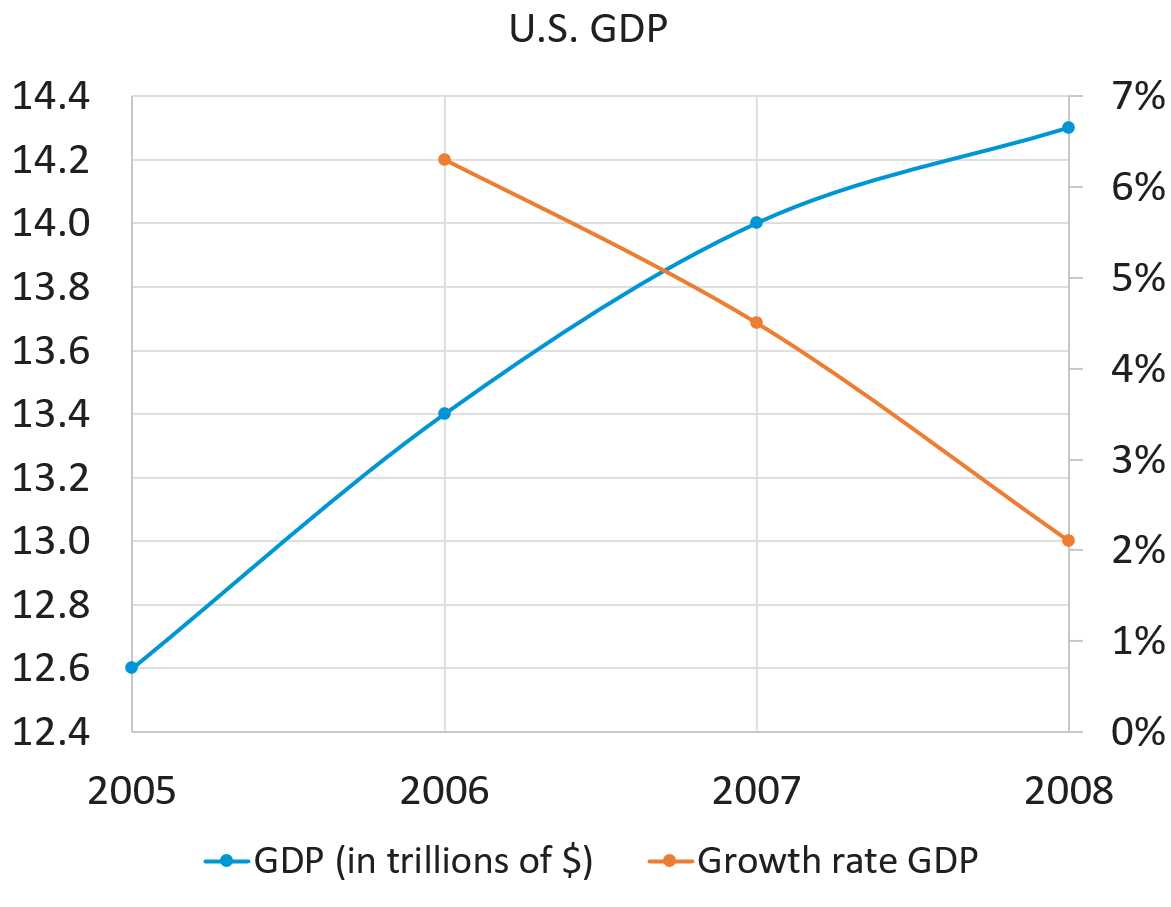
\includegraphics[width=0.7\linewidth]{Figures/screenshot001}
%			\end{figure}
%			
%		\end{column}%
%	\end{columns}
%\end{frame}


\begin{frame}[wide]{Measuring the State of the Economy}
	Gross domestic product (GDP): The market value of the final goods and services produced in an economy over a certain period
	\vspace{2mm}
	\begin{itemize}
		\item Production measure of GDP: The number of goods produced in the economy
		\item Expenditure measure of GDP: The total purchases in the economy
		\item Income measure of GDP: All the income earned in the economy
		\item All three approaches give identical measures of GDP:
		\[\mbox{Production} = \mbox{Expenditures} = \mbox{Income}\]
		\begin{itemize}
			\item This equation should hold in the ideal condition, but, in practice, measurement error, among other factors, cause these measures to be slightly different
		\end{itemize}
	\end{itemize}
\end{frame}

\begin{frame}[wide]{The Expenditure Approach to GDP}
	\begin{itemize}
		\item The national income accounting identity states: 
		\[Y= C+I+G+NX\]
		where
		\begin{itemize}[]
			\item $Y=$ GDP
			\item $C=$ consumption
			\item $I=$ Investment
			\item $G=$ Government purchases
			\item $NX=X-M=$ Export - Imports
		\end{itemize}
		\item This is probably one of the most important identity in Macroeconomics
		\item Only final good and service would be counted
	\end{itemize}
\end{frame}

\begin{frame}[wide]{Investment}
	\begin{itemize}
		\item Business fixed investment (non-residential)
		\begin{itemize}
			\item Spending by firms on plants, machinery and equipment
		\end{itemize}
		
		\item Residential investment 
		\begin{itemize}
			\item Construction of new houses and apartment buildings
			\item However, rent and old home resales enter into GDP through consumption as housing services produced
			\item Even if you own your house and don’t pay rent, you still receive “housing services.” 		Therefore, the value of housing imputed (estimated): what you would pay if you rented.
			
		\end{itemize}
		
	\end{itemize}
\end{frame}

\begin{frame}[wide]{Investment}
	\begin{itemize}
		\item Inventory investment
		\begin{itemize}
			\item Changes in inventories (of final or intermediate goods)
			\item Inventories are goods that are produced but not yet sold
			\begin{itemize}
				\item When there is an increase in inventories, this is treated as if the firm purchases these goods from themselves and are included in GDP
				\item Later, when inventories are sold as final goods, this results in a decrease in inventories (GDP) and an increase in consumption (also included in GDP)
			\end{itemize}
		\end{itemize}
		
	\end{itemize}
\end{frame}

\begin{frame}[wide]{Example of a National Account, US 2018}
	\begin{figure}
		\centering
		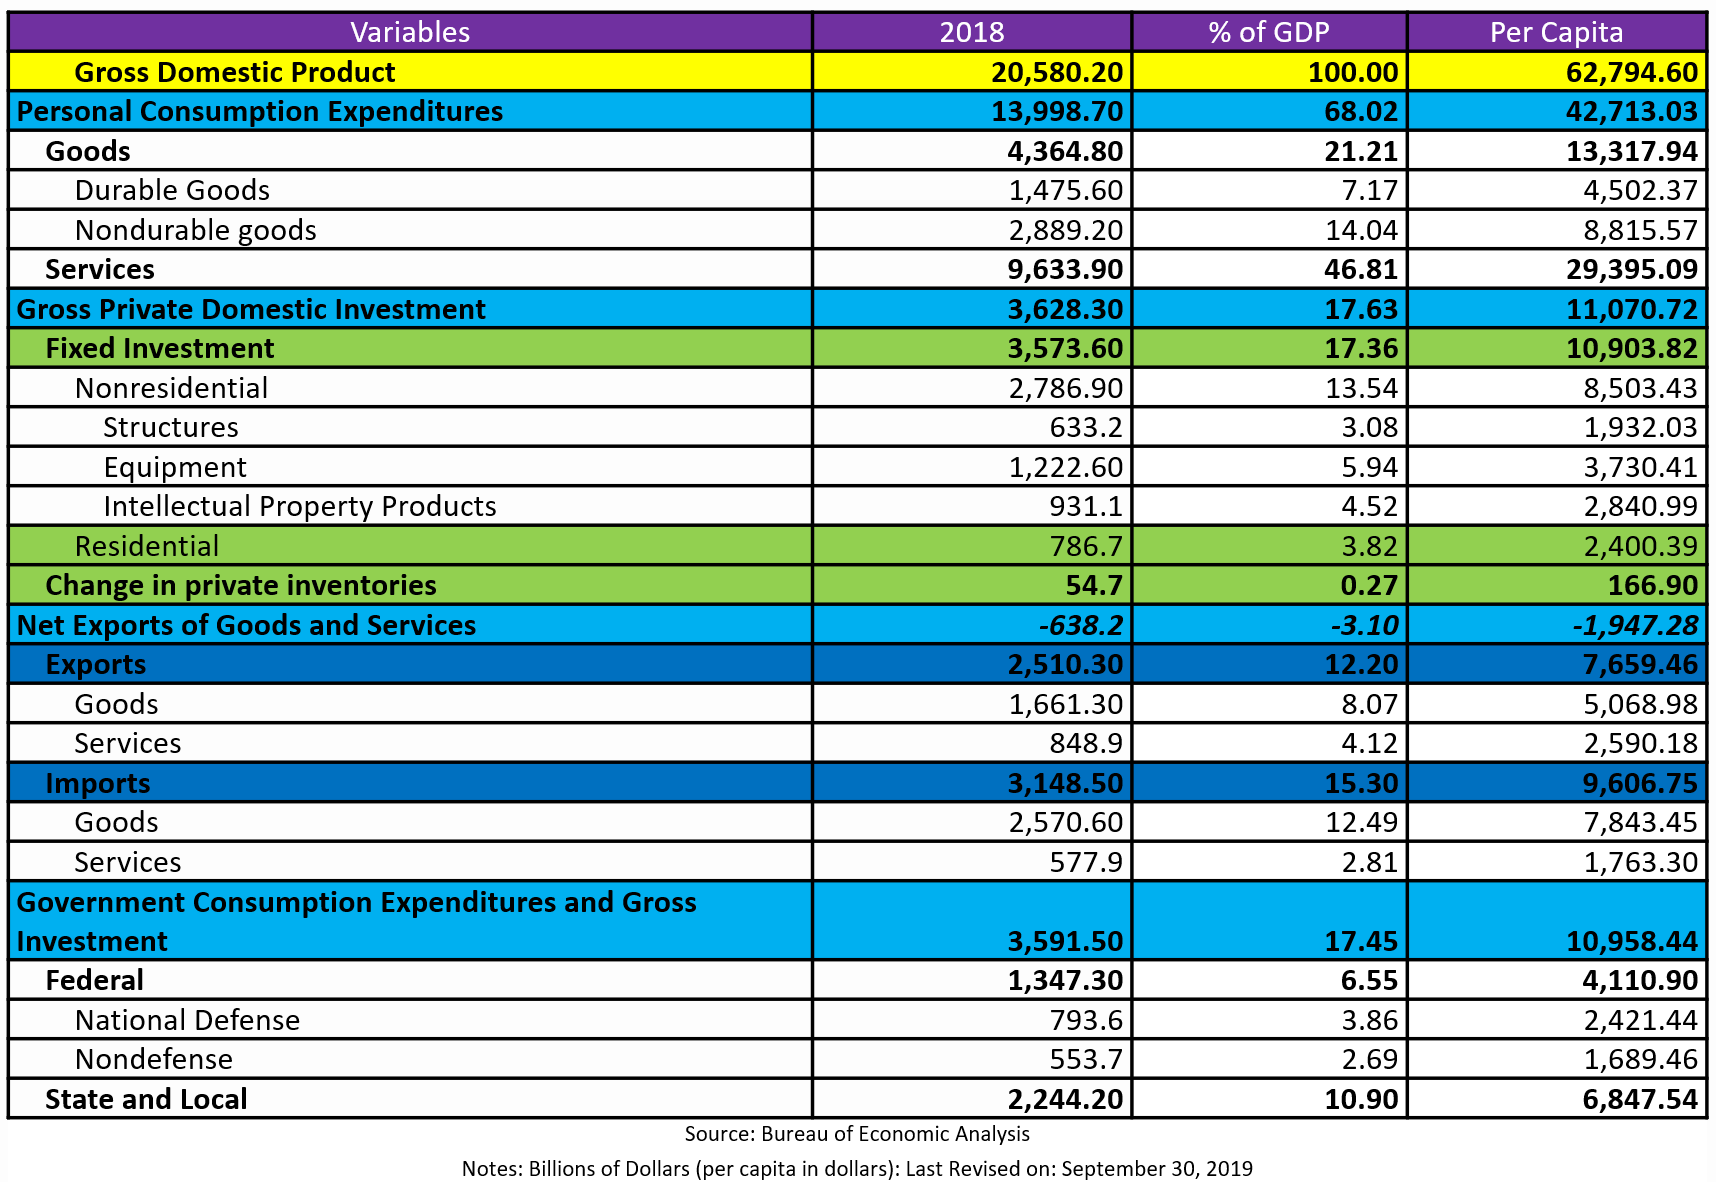
\includegraphics[width=0.8\linewidth]{Figures/national_account}
	\end{figure}
\end{frame}

\begin{frame}[wide]{Expenditure Shares of U.S. GDP}
	\begin{itemize}
		\item The composition of GDP has been relatively stable over time
		\item Consumption has increased as a share of GDP recently 
		\begin{itemize}
			\item NX being significantly negative
			\item Decline in government purchases 
		\end{itemize}
		\begin{figure}
			\centering
			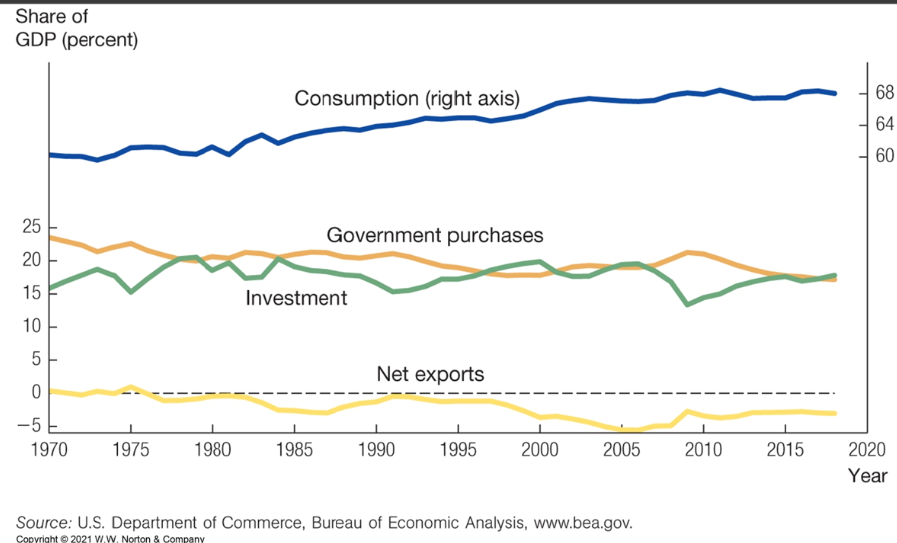
\includegraphics[width=0.65\linewidth]{Figures/national_account1}
		\end{figure}
		
	\end{itemize}
\end{frame}

\begin{frame}[wide]{The Income Approach to GDP}
	\begin{itemize}
		\item The income approach: 	Measures the sum of all income earned in the economy - from both labor and capital
		\item For every dollar of product sold there is a dollar of income earned
		\item Capital: 
		\begin{itemize}
			\item Inputs into production other than labor that are not used up in the production process
			\begin{itemize}
				\item Consider the cafe as an example: the coffee beans are not considered capital, but the coffee machine is regarded as a capital asset
			\end{itemize}
			\item Increased by firms through investment
		\end{itemize}
		\item Depreciation:	The deterioration of the capital stock due to wear and tear
		\[\mbox{GDP} - \mbox{depreciation}= \mbox{net domestic product} \]
	\end{itemize}
\end{frame}

\begin{frame}[wide]{The Income Approach to U.S. GDP in 2022}
	\begin{itemize}
		\item The majority of income (53 percent) comes from compensation to employees
		\item The next largest category is the net operating surplus of businesses -- “profits” earned by business owners, which provide both labour and capital
		\begin{figure}
			\centering
			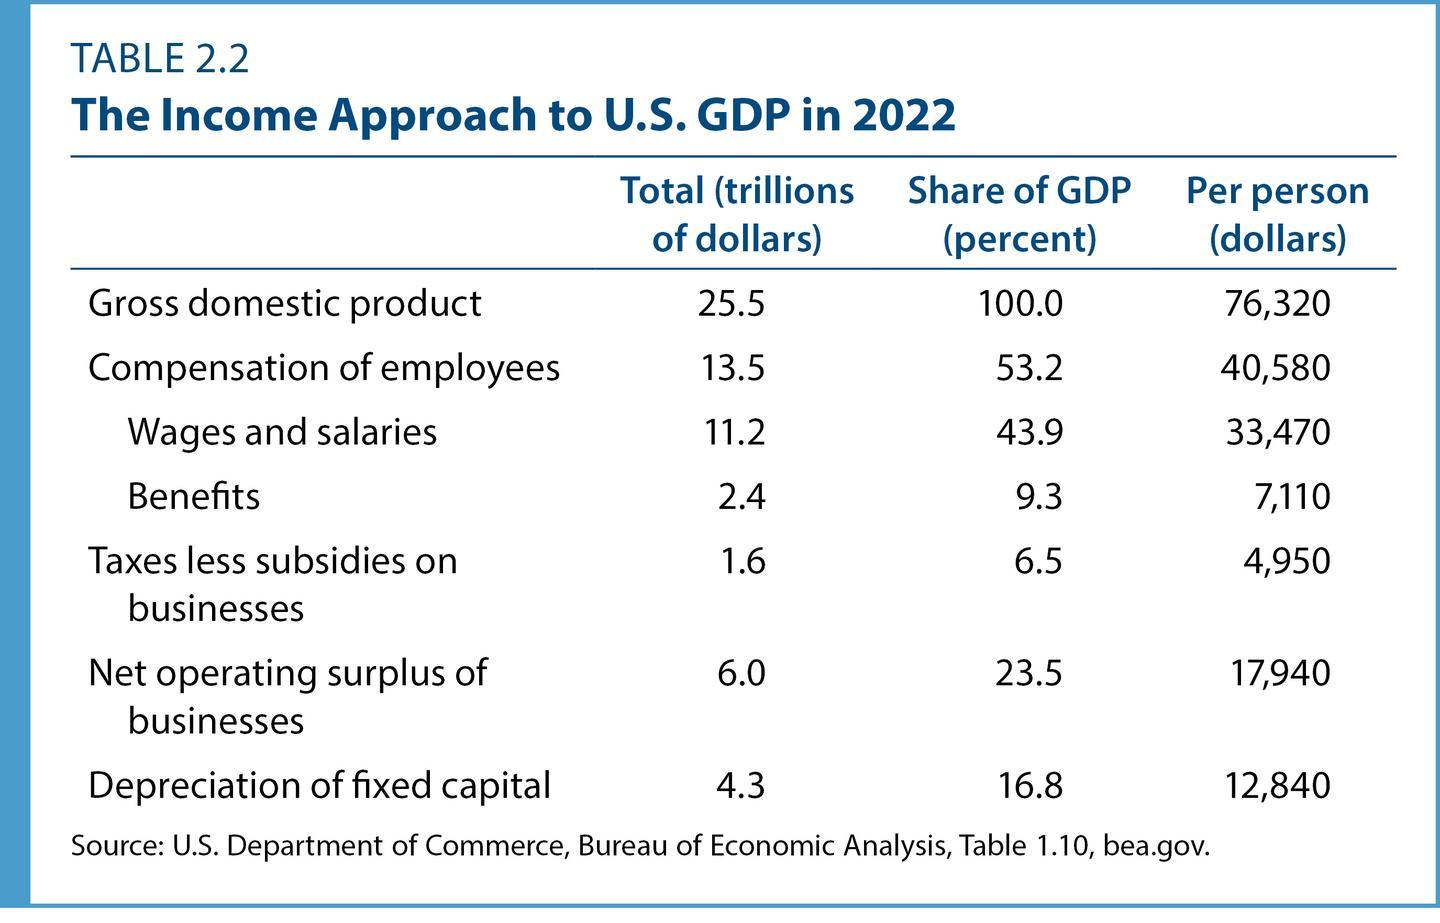
\includegraphics[width=0.7\linewidth]{Figures/Income_appoarch}
		\end{figure}
		
	\end{itemize}
\end{frame}

\begin{frame}[wide]{Total Share of GDP to Inputs}
	\begin{itemize}
		\item A convenient way to present this number is to split  income into labour income and capital income
		\item After adjusting the mixed income (income that involve both labour and capital), 
		\begin{itemize}
			\item Share of GDP to labour: Two-thirds (approx.)
			\item Share of GDP to capital: One-third (approx.)
		\end{itemize}
		
	\end{itemize}
\end{frame}

\begin{frame}[wide]{Labor’s Share of GDP}
	\begin{itemize}
		\item Notice that labor’s share of income fluctuates very little over time: between 60 and 70 percent of GDP
		\item There is no real general trend to labor’s share of income, but maybe we are the tipping point of falling in labour share
		\begin{itemize}
			\item In other words, it is not the case that capital owners are becoming richer at the expense of labor, or vice versa
		\end{itemize}		
		\begin{figure}
			\centering
			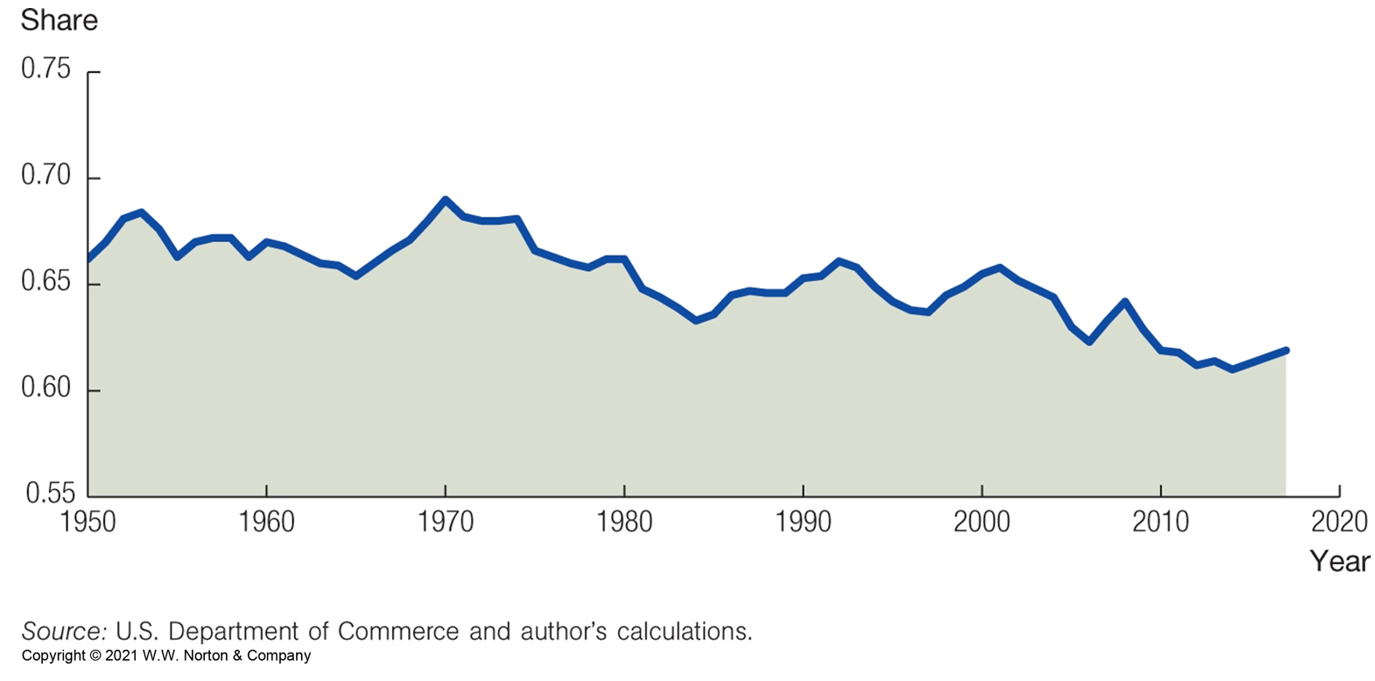
\includegraphics[width=0.7\linewidth]{Figures/labour_share}
		\end{figure}
		
	\end{itemize}
\end{frame}

\begin{frame}[wide]{The Production Approach to GDP}
	\begin{itemize}
		\item Recall that GDP is the value of final goods and services produced in an economy during a given period
		\begin{itemize}
			\item Do not want “double counting” in GDP
			\item If a steel company produces \$10 million worth of steel and that steel is then used by an automobile company to make \$100 million worth of cars:
			\begin{itemize}
				\item The value of the steel should not be counted twice
				\item GDP goes up by only \$100 million (the value of the final car sale)
			\end{itemize}
		\end{itemize}
		\item Value added
		\begin{itemize}
			\item The amount each producer contributes to GDP
			\item The revenue generated by each producer minus the value of intermediate products
		\end{itemize}
		\item Only new production of goods and services counts toward GDP
	\end{itemize}
\end{frame}

\begin{frame}[wide]{A Hypothetical Case}
	\begin{table}[htbp]
		\centering
		%		\caption{Add caption}
		\begin{tabular}{l|rrr|r}
			\multicolumn{1}{r}{} & \multicolumn{1}{l}{AT Cotton } & \multicolumn{1}{l}{ST Fabric} & \multicolumn{1}{l}{Savage Clothing} & \multicolumn{1}{l}{Total Factor Income} \\
			\midrule
			Value of sales & 3500  & 8000  & \cellcolor[rgb]{ 1,  1,  0}16000 &  \\
			\midrule
			Intermediate goods &       & 3500  & 8000  &  \\
			Wages & 1500  & 2000  & 2500  & \cellcolor[rgb]{ 1,  0,  0}6000 \\
			Interest & 200   & 400   & 600   & \cellcolor[rgb]{ 1,  0,  0}1200 \\
			Rent  & 800   & 1200  & 1600  & \cellcolor[rgb]{ 1,  0,  0}3600 \\
			Profit & 1000  & 900   & 3300  & \cellcolor[rgb]{ 1,  0,  0}5200 \\
			Total expenditure & 3500  & 8000  & 16000 &  \\
			\midrule
			Value added  & \cellcolor[rgb]{ .573,  .816,  .314}3500 & \cellcolor[rgb]{ .573,  .816,  .314}4500 & \cellcolor[rgb]{ .573,  .816,  .314}8000 &  \\
		\end{tabular}%
	\end{table}%
	\begin{itemize}
		\item For this simple economy, the GDP can be calculated in three approaches
		\item Summing the all the red cell give the income approach GDP, green give the value added approach, and yellow gives the expenditure approach
	\end{itemize}
\end{frame}

\begin{frame}[wide]{What Is Included in GDP and What Is Not?}
	\begin{itemize}
		\item Included:
		\begin{itemize}
			\item Government spending on goods/services
			\item Factory production
			\item Healthcare expenditures
			\item Ingredients and food purchased
			\item Kids in day care
		\end{itemize}
		\item Not included:
		\begin{itemize}
			\item Government transfer payments
			\item Environmental conditions
			\item A measure of a nation’s health 
			\begin{itemize}
				\item See: https://www.gapminder.org/videos/200-years-that-changed-the-world/
			\end{itemize}
			\item Time spent cooking at home
			\item Babysitter
		\end{itemize}
		
	\end{itemize}
\end{frame}

\begin{frame}[wide]{Beyond GDP}
	\begin{itemize}
		\item GDP is used by economists as a proxy for standards of living, but economist want to create broader measure
		\item Jones and Klenow (2016) started with looking at consumption per person instead of production
		\item Motivated by the typical building board in macroeconomics and in microeconomics, they also incorporate life expectancy, leisure and consumption inequality in to the analysis
	\end{itemize}
\end{frame}

\begin{frame}[wide]{Beyond GDP: GDP and Welfare across Countries in Year 2007}
	% Table generated by Excel2LaTeX from sheet 'Sheet1'
	\begin{table}[htbp]
		\centering
		\begin{tabular}{lcccccc}
			&       &       & \multicolumn{4}{c}{Decomposition} \\
			\cmidrule{4-7}          & Per capita &       & Life  &       &       &  \\
			Country & GDP   & Welfare & Expectancy & C/Y   & Leisure & Inequality \\
			\midrule
			US    & 100   & 100   & 0     & 0     & 0     & 0 \\
			&       &       & 77.8  & 0.845 & 836   & 0.658 \\
			Sweden & 79.4  & 91.2  & 0.181 & -0.186 & 0.01  & 0.135 \\
			&       &       & 80.9  & 0.701 & 807   & 0.404 \\
			Japan & 71.3  & 82.6  & 0.265 & -0.154 & -0.028 & 0.063 \\
			&       &       & 82.5  & 0.724 & 912   & 0.554 \\
			South Korea & 58.3  & 45.3  & 0.078 & -0.29 & -0.116 & 0.076 \\
			&       &       & 79.3  & 0.632 & 1120  & 0.531 \\
			Vietnam & 5.9   & 4     & -0.082 & -0.269 & -0.02 & -0.006 \\
			&       &       & 74.2  & 0.645 & 893   & 0.668 \\
			Kenya & 2.8   & 1.9   & -0.394 & 0.104 & 0.059 & -0.157 \\
			&       &       & 54.4  & 0.938 & 644   & 0.865 \\
			\bottomrule
		\end{tabular}%
	\end{table}%
	The US's per capita GDP and welfare are normalized to 100
\end{frame}

\begin{frame}[wide]{Measuring Changes Over Time}
	\begin{itemize}
		\item When examining GDP over time, we need to take into account changes in prices
		\item Nominal GDP: 	A measure of GDP when prices and quantities have not been separated, using current year prices
		\begin{itemize}
			\item Nominal GDP = $\mbox{price level} \times \mbox{Real GDP}$
			\item If prices are increasing over time, then GDP will increase, regardless of whether or not there is an increase in quantity.
			
		\end{itemize}
		\item Real GDP: Actual quantity of goods and services, using base year prices
		\begin{itemize}
			\item Real GDP = $\frac{\mbox{Nominal GDP}}{\mbox{Price Level}}$
		\end{itemize}
	\end{itemize}
\end{frame}

\begin{frame}[wide]{Measuring Changes Over Time}
	\begin{itemize}
	\item To compute GDP across time, we must use a certain year’s prices.
	\begin{itemize}
		\item 	Real GDP will be measured in a certain year’s dollars
		\item Nominal GDP is measured in current dollars
	\end{itemize}
	\item Think of there are $N$ different good/service in the economy, each of them have their own price
	\item Nominal GDP: $Y_t= P_{1,t} Q_{1,t} + P_{2,t} Q_{2,t} + \dots + P_{N,t} Q_{N,t}$
	where $N$ is the total number of goods and services in the economy and $P_{i,t} $ are prices of good $i$ in year $t$
	\item Real GDP: $Y_t = P_{1,b} Q_{1,t} + P_{2,b} Q_{2,t} + \dots + P_{N,b} Q_{N,t}$
	where $P_{i,b}$ is the price of good $i$ in the base year
	\end{itemize}
\end{frame}

\begin{frame}[wide]{An Example of Changes in Nominal GDP}
	\begin{itemize}
		\item Consider an economy that produces two goods: donuts (d) and pizza (p).
		\item Nominal GDP in 2020:
		\[Y_{2020} = P_{d,2020} Q_{d,2020} + P_{p,2020} Q_{p,2020}\]
		\item Real GDP in 2020 (base year = 2014):
		\[Y^R_{2020} = P_{d,2014} Q_{d,2020} + P_{p,2014} Q_{p,2020}\]
		\item If the quantity of goods and services produced does not change, but prices do change:
		\begin{itemize}
			\item Nominal GDP will change
			\item Real GDP will not change
		\end{itemize}
	\end{itemize}
\end{frame}

\begin{frame}[wide]{An Example of Changes in Nominal GDP}
	\begin{table}[htbp]
		\centering
		\begin{tabular}{lcccc}
			Year  & Price of  & Quantity of  & Price of  & Quantity of  \\
			& Donuts &  Donuts &  Pizza & Pizza \\
			\midrule
			2014 (base) & 10    & 50    & 25    & 100 \\
			2015  & 12    & 50    & 28    & 100 \\
			\bottomrule
		\end{tabular}%
	\end{table}%
	\begin{itemize}
		\item Nominal GDP in 2014 $= 10\times 50 + 25 \times 100 = 3000$
		\item Nominal GDP in 2015 $= 12 \times 50 + 28 \times 100 = 3225$
		\item Real GDP in 2015 $= 10 \times 50 + 25 \times 100 = 3000$
		\item The real GDP in 2015 is the same as the nominal GDP in 2014, because only the price has increased
	\end{itemize}
\end{frame}

\begin{frame}[wide]{An Example of Changes in Nominal GDP}
	\begin{table}[htbp]
		\centering
		\begin{tabular}{lcccc}
			Year  & Price of  & Quantity of  & Price of  & Quantity of  \\
			& Donuts &  Donuts &  Pizza & Pizza \\
			\midrule
			2014 (base) & 10    & 50    & 25    & 100 \\
			2015  & 12    & 55    & 28    & 105 \\
			\bottomrule
		\end{tabular}%
	\end{table}%
	\begin{itemize}
		\item Nominal GDP in 2015 $= 12 \times 55 + 28 \times 105 = 3660$
		\item Real GDP in 2015 $= 10 \times 55 + 25 \times 105 = 3175$
	\end{itemize}
\end{frame}

\begin{frame}[wide]{Another Calculation}
	\begin{figure}
		\centering
		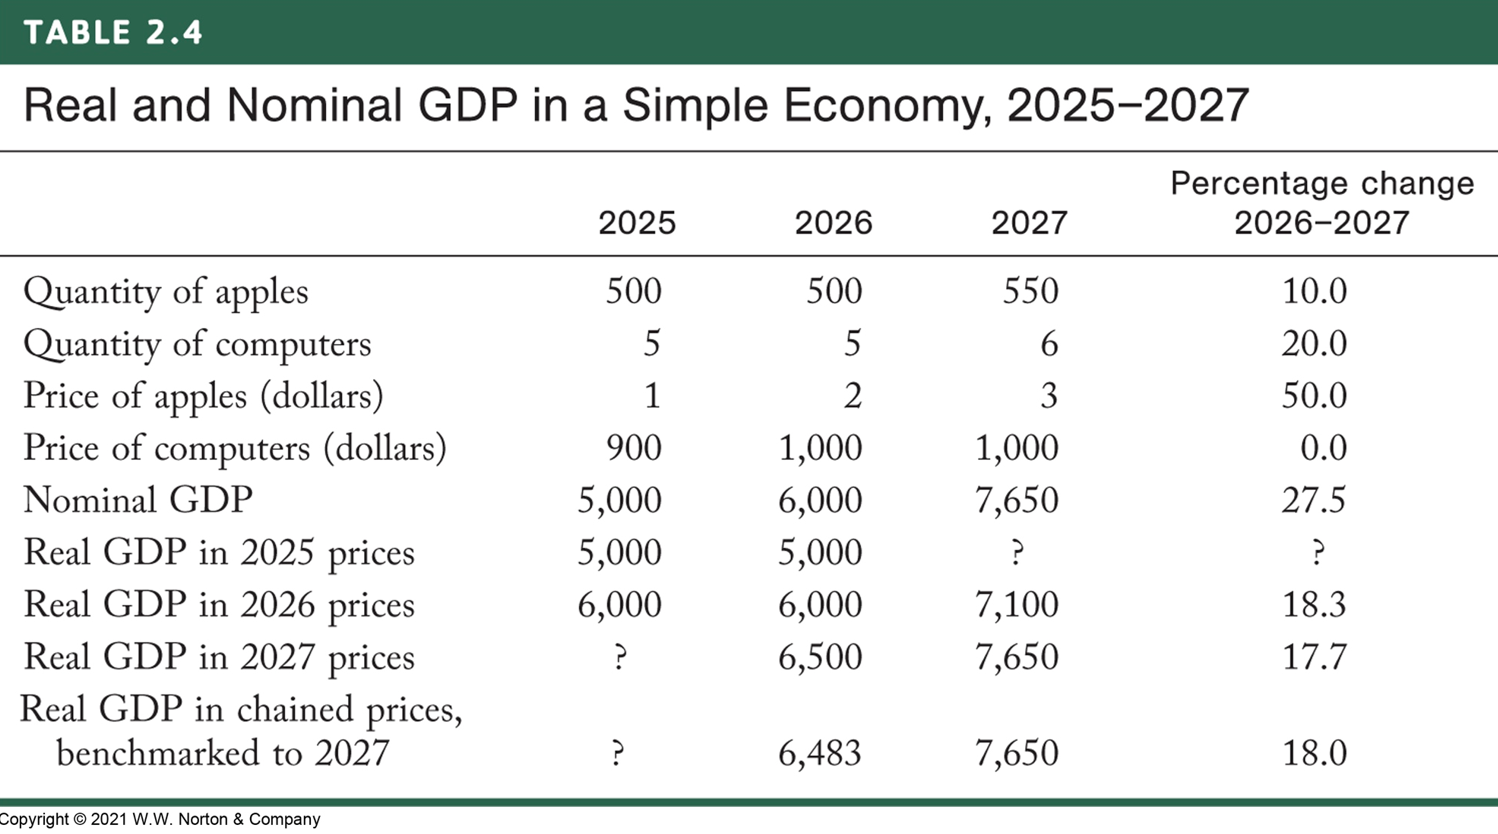
\includegraphics[width=0.9\linewidth]{Figures/GDP_calculation}
	\end{figure}
\end{frame}

\begin{frame}[wide]{Quantity Indexes}
	Calculating real GDP changes over time:
	\begin{itemize}
		\item The Laspeyres index: 	Calculates changes in real GDP using the initial prices
		\begin{itemize}
			\item e.g., for year 2026 to 2027, 
			\[\mbox{Laspeyres index} = \frac{7100}{6000} = 1.183\]
		\end{itemize}
		\item The Paasche index: Calculates changes in real GDP using the final year prices
		\begin{itemize}
			\item e.g., for year 2026 to 2027, 
			\[\mbox{Paasche index} = \frac{7650}{6500}=1.177\]
		\end{itemize}
		\item We can multiply the index by 100 so it is easier to read, but it is not required
		\item Over long-time intervals the two indexes can result in substantial differences
	\end{itemize}
\end{frame}

\begin{frame}[wide]{Chain Weighting}
	\begin{itemize}
		\item The Fisher index (chain weighting) is the preferred approach to calculating real GDP
		\begin{itemize}
			\item Geometric Average of the Laspeyres and Paasche index
				\[\mbox{Fisher Index} = \sqrt{\mbox{Laspeyres} \times \mbox{Paasche}}\]
			\item 
		\end{itemize}
		\item It is preferred because new goods are invented while others become obsolete, using only early or recent prices would be inaccurate.
		\item In the example above, we have the fisher index $=\sqrt{118.3\times 117.7} = 118$ or in growth rate $118/100 -1 = 18\%$
		\[Y^F_{2026} \times 1.18= 7650 \to Y^F_{2026} = 7650/1.18 = 6483\]
	\end{itemize}
\end{frame}

\begin{frame}[wide]{Chain Weighting}
	\begin{itemize}
		\item To calculate the 2025 real GDP in chained prices, benchmarked to 2027, we have to calculate the following:
		
		Let $G_{26,27}$ be the growth rate of the fisher index between year 26 to 27
		
		\[Y^F_{2025} G_{25,26}\times G_{26,27} = Y^F_{2027}\]
		
		We have calculate $G_{26,27}$ already, which is equal to $0.18$
		
		\item Now we have to calculate $G_{25,26}$. From the table, we know that there is no real growth between these two years. Therefore, 
		\[G_{25,26} = \sqrt{\frac{6000}{6000} \times \frac{5000}{5000}} = 1\]
		
		\item Last, rearrange the equation above
		\[Y^F_{2025}  = \frac{Y^F_{2027}}{G_{25,26}\times G_{26,27}} = \frac{7650}{1.18} = 6483\]
		This is the same as the number in year 2026
	\end{itemize}
\end{frame}

\begin{frame}[wide]{GDP Deflator}
	\begin{itemize}
		\item Recall that 
		\[\mbox{Nominal GDP} = \mbox{Price level} \times \mbox{real GDP}\]
		Rearrange that
		\[\mbox{Price level} = \frac{\mbox{Nominal GDP}}{\mbox{real GDP}} \]
		\item This measure is called the GDP deflator
		\item Similar deflators exist for the various components of GDP, such as consumption and investment
	\end{itemize}
\end{frame}

\begin{frame}[wide]{Price Indexes and Inflation}
	\begin{itemize}
		\item We can consider the following transformation:
		\[\%\Delta \mbox{Nominal GDP} \approx \%\Delta \mbox{Price}+ \%\Delta \mbox{real GDP}\]
		This approximation hold if the change is relatively small
		\item If the $\%\Delta \mbox{Nominal GDP} = 27.5\%$ and the $\%\Delta \mbox{real GDP} = 18\%$, the percentage change in price is $9.5\%$
		\item The percentage change in price is also called inflation rate
	\end{itemize}
\end{frame}

\begin{frame}[wide]{Using Chain-Weighted Data}
	\begin{itemize}
		\item Main motive for chain-weighted data: Rapid price changes in computer industry during the 1990s
		\begin{itemize}
			\item The difference between the two indexes widen
		\end{itemize}
		\item Main disadvantage:
		\begin{itemize}
			\item The sum of real C, I, G, NX will not equal real chain-weighted GDP because the prices used in constructing the components are different
		\end{itemize}
		\item General rule to follow:
		\begin{itemize}
			\item For particular components of GDP, we look at the ratio of nominal variables
			\item When you want real rates of economic growth, use the chain-weighted real measures
		\end{itemize}
	\end{itemize}
\end{frame}

\begin{frame}[wide]{Comparing Economic Performance across Countries}
	\begin{itemize}
		\item The exchange rate:
		\begin{itemize}
			\item Represents the price at which various currencies are exchanged
		\end{itemize}
		\item When comparing GDP across countries:
		\begin{itemize}
			\item It is essential to express GDP in a common currency by adjusting it using the exchange rate
			\item The resulting nominal GDP should then be further multiplied by the ratio of price levels in the respective countries
		\end{itemize}
		\item World Bank and Penn World Tables are the two common source for exchange rate and price level adjusted data
	\end{itemize}
\end{frame}

\begin{frame}[wide]{An Example of Comparisons of Economies}
	Suppose we are trying to compare GDP in Canada and the United States. 
	\begin{itemize}
		\item Use the exchange rate to turn Canadian dollars into U.S. dollars:
		\[2.316 \mbox{Trillion CAD}\times \frac{1}{1.327} = 1.745 \mbox{Trillion USD}\]
		\item Adjust for relative price level of goods :
		\[1.745 \mbox{Trillion USD} \times  \frac{1}{0.935} =  1.866 \mbox{Trillion USD}\]
		\item 
		\[\mbox{Real GDP}^{\mbox{US-price}}_{\mbox{CA}}  = \mbox{price level}_{US} \times \mbox{real GDP}_{CA} = \mbox{price level}_{US} \times \frac{\mbox{nominal GDP}_{CA}}{\mbox{Price Level}_{CA}}\]
		\[  = \frac{\mbox{price level}_{US}}{\mbox{Price Level}_{CA}} \times \mbox{nominal GDP}_{CA}\]
		The term $\frac{\mbox{price level}_{US}}{\mbox{Price Level}_{CA}} = \frac{1}{0.935}$ and $\mbox{nominal GDP}_{CA} = 1.745 \mbox{Trillion USD}$
	\end{itemize}
\end{frame}

\begin{frame}[wide]{Comparison of Countries}
	\begin{itemize}
		\item In general, rich countries tend to have higher price levels than poor countries
		\item This is mainly because poor countries have lower wages
		
	\end{itemize}
\end{frame}

\begin{frame}[wide]{Next Lecture}
	\begin{itemize}
		\item Next lecture will cover Ch.3
	\end{itemize}
\end{frame}

\end{document}